\documentclass[10pt, a4paper]{article}

%%%%%%%%%%%%%%
%  Packages  %
%%%%%%%%%%%%%%


\usepackage{page_format}
\usepackage{special}
\usepackage{hyperref}
\usepackage{tikz}
\usepackage{pgfplots}
\usepackage[compat=1.1.0]{tikz-feynman}
\usepackage[font=small,labelfont=bf,
   justification=justified,
   format=plain]{caption}
\input{math_func}

\usepackage{slashed}

% References
\usepackage{biblatex}
\addbibresource{ref.bib}
\usetikzlibrary{intersections}

%%%%%%%%%%%%
%  Colors  %
%%%%%%%%%%%%
% ! EDIT HERE !
\colorlet{chaptercolor}{red!70!black} % Foreground color.
\colorlet{chaptercolorback}{red!10!white} % Background color

%%%%%%%%%%%%%%
% Page titre %
%%%%%%%%%%%%%%%
\title{Homework 3: Interstellar's Ring} % Title of the assignement.
\author{\PA} % Your name(s).
\teacher{Ruth Gregory} % Your teacher's name.
\class{Gravitational Physics} % The class title.

\university{Perimeter Institute for Theoretical Physics} % University
\faculty{Perimeter Scholars International} % Faculty 
%\departement{<Departement>} % Departement
\date{\today} % Date.


%%%%%%%%%%%%%%%%%%%%%%
% Begin the document %
%%%%%%%%%%%%%%%%%%%%%%
\begin{document}

% Make the title page.
\maketitlepage

% Make table of contents
\maketableofcontents

% Assignment starts here ----------------------------

\section{Setup}
We are interested in describing a Schwarzchild black hole of mass $M$ described by the Schwarzchild coordinates $(t', r', \theta', \phi')$. In this coordinate system, the singularity of the black hole is approached as $r' \to 0$ and the event horizon is the null hypersurface with $r' = 2GM + R_S$. The rotational symmetry of the system is broken by adding an accretion disk of external radius $a$ orbiting in the $\theta = \pi/2$ equatorial plane of the Schwarzchild coordinates. We are interested in the image of the light created by the accretion disk as seen by an observer at $r'\to \infty$. This observer will carry a local Minkowski coordinate system $(t, x, y, z)$. We take $t = t'$ forcing the observer to be static with respect to the black hole (using an infinitesimal acceleration to cancel its geodesic flow towards the black hole). The remaining coordinates $x, y, z$ are related to the asymptotic Schwarzchild coordinates $x', y', z'$ (respectively given by $r' \sin \theta' \cos \phi', r' \sin \theta' \sin \phi', \text{ and } r'\cos \theta'$) by a rotation. This rotation is fixed by taking $x = x'$ as the rotation axis and orienting the $z$ axis in the direction of the observer (note that this implies that the radius coordinate value $r = \sqrt{x^2 + y^2 + z^2} = r'$ is shared between the two systems, but refer to very different metrics at small $r$). The angle between $z$ and $z'$ is denoted $\theta_0$. 

The image at $r\to \infty$ is generated by the collection of light geodesic crossing the $xy$ plane parallel to the $z$ axis. For a given crossing point on the $xy$-plane we can time reverse (parameter reverse is more appropriate since the geodesic is null) the geodesic motion to see if this point is associated with an accretion disk initial condition and light the crossing point accordingly. The location of the crossing point on the $xy$ plane is identified with an angle $\phi = \text{arctan}_2(y, x)$ and a radius $b$ (the impact parameter of the geodesic at $r\to \infty$). An important feature of Schwarzchild geodesics is that they are planar: if the geodesic starts at an angle $\phi'$ on the accretion disk it will stay at the same angle. For a given impact parameter $b$ at angle $\phi$, there is a point of maximal approach to the black hole (periastron) with radius $r = r_0(b, \phi)$.  


\section{Warm up}
To better study geodesics around a Schwarzchild black hole, we use a different set of Schwarzchild coordinates $(t, r, \chi, \psi)$ (with the same time coordinate as the initial coordinate system) to simplify the calculations in the plane of motion. More precisely the plane of motion constitutes the equatorial plane $\chi = \pi/2$ of the coordinate system. Projecting all points of the geodesic on a constant $t$ slice, expressed in the polar coordinates $r, \psi$
of the equatorial plane. Finally, the $\psi = 0$ direction is aligned with the rays reaching the observer. 

\begin{enumerate}
  \item[(a)] Figure \ref{fig1} shows sketches of three geodesics in an equatorial plane orthogonal to the accretion disk. The red geodesic has an impact parameter $b$ such that the point of the accretion disc plane reached by moving backward in the parameter is out of the accretion disc. Geodesics $1$ and $2$ correspond to light reaching the observer. They have different periastra $r_0^1$ and $r_0^2$ and different impact parameters.
  \begin{figure}[h!]
    \centering
    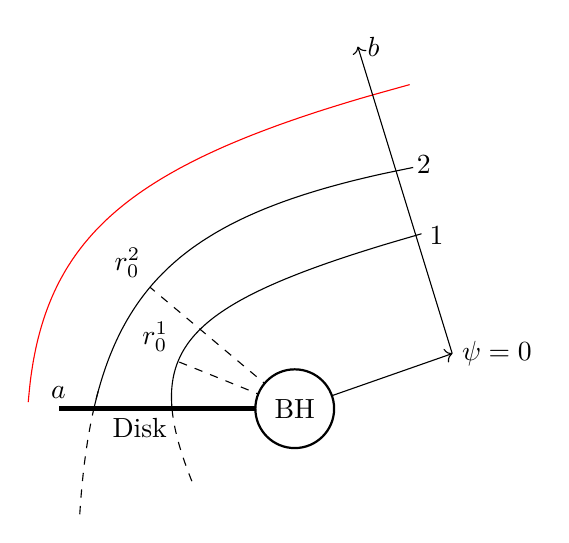
\begin{tikzpicture}[scale=2, rotate=0]
    
      % Define hyperbola parameters
      \def\a{1.2}
      \def\b{0.8}
      \def\c{-1}
    
      % Draw the hyperbola
      \draw[rotate=-22, dashed] plot[smooth,domain=-40:-19] ({\a*sec(\x)-2},{\b*tan(\x)});
      \draw[rotate=-40, dashed] plot[smooth,domain=-40:-22] ({1.5*\a*sec(\x-1) + \c -2},{2*\b*tan(\x-1)});
      \draw[rotate=-22] plot[smooth,domain=-19.5:59] ({\a*sec(\x)-2},{\b*tan(\x)});
      \draw[rotate=-40] plot[smooth,domain=-26:47] ({1.5*\a*sec(\x-1) + \c -2},{2*\b*tan(\x-1)});
      \draw[ultra thick] (0, 0) -- (-1.5, 0);
      \draw[rotate=-22, dashed] (0, 0) -- (-0.8, 0) node[above left] {$r_0^1$};
      \draw[rotate=-40, dashed] (0, 0) -- (-1.5 * 0.8, 0) node[above left] {$r_0^2$};

      \draw[rotate=-33, red] plot[smooth,domain=-28:54] ({1.5*\a*sec(\x-1) + \c -2.5},{2*\b*tan(\x-1)});

      \draw[->] (0, 0) -- (1, 0.35) node[right] {$\psi = 0$};
      \draw[fill=white, thick] (0,0) circle [radius=0.25];

      \draw (0.9,1.1) node {$1$};
      \draw (0.82,1+0.55) node {$2$};
      \draw (-1.5,0) node[above ] {$a$};
      \draw (-1.5/2,0) node[below left] {Disk};

      \draw[->] (1, 0.35) -- (3*0.8-3+1, 3-3*0.35+0.35) node[right] {$b$};
      
      \draw (0,0) node {BH};
    \end{tikzpicture}
    \caption{Equatorial plane sketch of geodesic motion with three different impact parameters and periastra \label{fig1}. The periastra gets further away from the accretion disk point as we get closer to the outer ring of the accretion disk. If the disk was large, the geodesic starting on the outer ring would approximatively be a straight line starting at the disk point and directed towards the observer. In this limit, the periastron is located exactly in the middle of the line. In this sketch the example geodesic are curving in the clockwise direction relative to the $\psi = 0$ axis. This is why Figures \ref{fig2} and \ref{fig3} are plotted against $-\psi$ (making the deflexion angles negative)}
  \end{figure}
\newpage
  \item[(b)] Figure \ref{fig2} compares the total deflexion angle for the two geodesics presented in \ref{fig1}.
  \begin{figure}[h!]
    \centering
    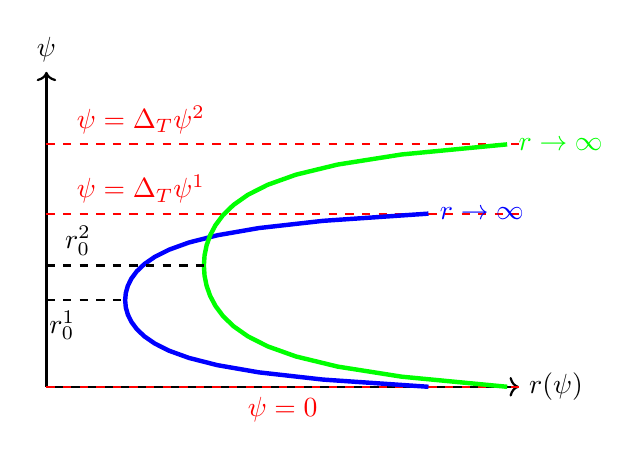
\begin{tikzpicture}[domain=-4:7] [scale=2]
      \draw[thick, ->] (0,0) -- (6,0) node[right] {$r(\psi)$};
      \draw[thick,->] (0,0) -- (0,4) node[above] {$\psi$}; %-
      \draw[thick, red, dashed] (0,.35*pi*2) -- (6,.35*pi*2) node[pos=0.2, above] {$\psi = \Delta_T \psi^1$};
      \draw[thick, red, dashed] (0,.35*pi*2*1.4) -- (6,.35*pi*2*1.4) node[pos=0.2, above] {$\psi = \Delta_T \psi^2$};
      \draw[thick, red, dashed] (0,0) -- (6,0) node[midway, below] {$\psi = 0$};
      \draw[ultra thick,color=blue] plot[domain=-.35*pi:.35*pi] ({1+tan(\x r)*tan(\x r)}, \x+0.35*pi) node[right] {$r\to \infty$};
      \draw[ultra thick,color=green] plot[domain=-.35*pi:.35*pi] ({2+tan(\x r)*tan(\x r)}, 1.4*\x+1.4*0.35*pi) node[right] {$r\to \infty$};
      \draw[thick, dashed] (0, 0.35*pi) -- (1, 0.35*pi) node[pos=0.2, below] {$r_0^1$};
      \draw[thick, dashed] (0, 1.4*0.35*pi) -- (2, 1.4*0.35*pi) node[pos=0.2, above] {$r_0^2$};
    \end{tikzpicture}
    \caption{$\psi$ coordinate describing geodesics $1$ (blue) and $2$ (green) from \ref{fig1} as a function of the respective radial coordinate $r$. The full geodesics (extended beyond the accretion disc) start at $r \to \infty$ and end again at $r\to \infty$. We choose $\psi = 0$ to represent the observer angle for both geodesic forcing them to coincide on the $\psi = 0$ axis. The other asymptote represents the extended initial direction of motion of light consistent with the initial accretion disc point. The minimal value of $r$ (the periastron) is realized in the middle of the geodesic motion. From the dashed lines in \ref{fig1}, we see that the total deflexion angle $\Delta_T \psi^{1, 2}$ between $\phi = 0$ and the extended motion asymptote is smaller for geodesic $1$ compared to geodesic $2$ (we have $\Delta_T \psi^{1} < \Delta_T \psi^{2}$). This is consistent with the increasing gravitational pull with decreasing pariastron. \label{fig2}}
  \end{figure}
  \item[(c)] Figure \ref{fig3} represents the same goedesics as figure \ref{fig2}, but has the radial coordinate $r$ replaced by the inverse radial coordinate $u = 1/r$.
  \begin{figure}[h!]
    \centering
    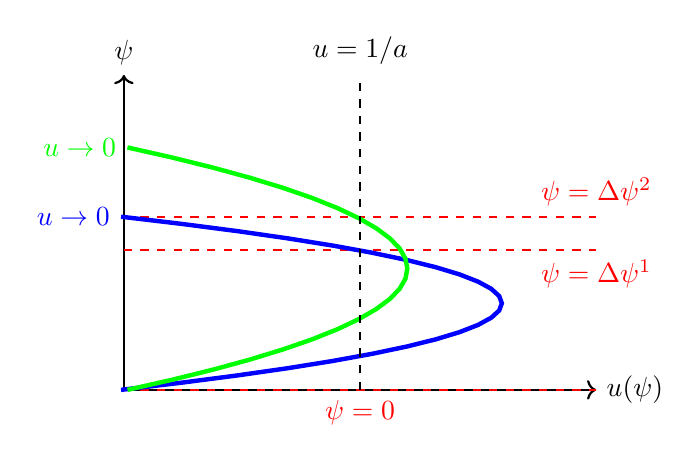
\begin{tikzpicture}[domain=-4:7] [scale=2]
      \draw[thick, ->] (0,0) -- (6,0) node[right] {$u(\psi)$};
      \draw[thick,->] (0,0) -- (0,4) node[above] {$\psi$};%-
      \draw[thick, red, dashed] (0,.35*pi*2) -- (6,.35*pi*2) node[pos=1, above] {$\psi = \Delta \psi^2$};
      \draw[thick, red, dashed] (0,.35*pi*2*1.4-1.3) -- (6,.35*pi*2*1.4-1.3) node[pos=1, below] {$\psi = \Delta \psi^1$};
      \draw[thick, red, dashed] (0,0) -- (6,0) node[midway, below] {$\psi = 0$};
      \draw[ultra thick,color=blue] plot[domain=-.35*pi:.35*pi] ({4*(0.2+1-\x*\x)}, \x+0.35*pi) node[left] {$u\to 0$};
      \draw[ultra thick,color=green] plot[domain=-.35*pi:.35*pi] ({1.5*(0.4+2-1.4*1.4*\x*\x)}, 1.4*\x+1.4*0.35*pi) node[left] {$u\to 0$};
      %\draw[thick, dashed] (0, 0.35*pi) -- (3*0.2+3, 0.35*pi) node[pos=0, left] {$u_0^1 = 1/r_0^1$};
      %\draw[thick, dashed] (0, 1.4*0.35*pi) -- (2.5*0.4+5, 1.4*0.35*pi) node[pos=0, left] {$u_0^2 = 1/r_0^2$};
      \draw[thick, dashed] (3, 0) -- (3, 4) node[pos=1, above] {$u = 1/a$};
    \end{tikzpicture}
    \caption{$\psi$ coordinate describing geodesics $1$ (blue) and $2$ (green) from \ref{fig1} as a function of the respective inverse radial coordinate $u = 1/r$. We define the partial deflexion angle $\Delta \psi^{1, 2}$ as the angle between the observer direction ($\psi = 0$) and the first crossing of the $u=1/a$ surface by the geodesic (accretion disk point). Since there are two crossing points, we have to specify which one corresponds to the disk. \label{fig3}}
  \end{figure}
  %Note: The convention used in the previous figures is different from the one used in the assignment. The assignment convention uses the extended motion initial asymptote as the $\psi=0$ direction. This implies that the total deflexion angle consistent with this convention is $-\Delta_T \psi^{1, 2}$ since it is measured between the same asymptotes, but in reversed order. The partial deflexion angle consistent with the assignment convention is $-(\Delta_T\psi^{1, 2}-\Delta\psi^{1, 2})$ where the global sign takes the relative orientations into account. Since the angles were negative because of the clockwise deflexions in figure \ref{fig1}, the assignment convention angles are positive for the same configuration. In what follows, we use the angle convention of the assignment. 
\end{enumerate}
% does this happen with stars ?
\newpage
\section{Null geodesics in a Schwarzchild's spacetime}
\begin{enumerate}
  \item[(a)] Using the killing vectors $\partial_{t'}$ and $\partial_{\phi'}$, we respectively obtain the conserved quantity $E$ and $L$ along the geodeics of the Schwarzchild spacetime. At $r' \to \infty$, these quantities become the Minkowski energy and orbital momentum of a free particle. For a massless particle, the energy at $r\to \infty$ is $E = p$ with $p$ the magnitude of the momentum. The magnitude of angular momentum is $L = p r_\perp$ where $r_\perp$ is the projection of the radial coordinate in the direction orthogonal to the geodesic asymptote in the plane of motion. We an identify  $b = r_\perp = L/E$. In equatorial plane $\chi = \pi/2$ of the $(t, u = 1/r, \chi, \psi)$ coordinate system, we use the affine parameter $\lambda$ to parametrize the geodesic as $(u(\lambda), \psi(\lambda))$. The geodesic equation satisfied by these coordinates is 
  \begin{align*}
    \dot{u}^2=E^2 b^2 u^4 U_{\text {eff }}(u), \quad \dot{\psi}=E b u^2 \quad \text{ where }\quad U_{\text {eff }}(u)=\frac{1}{b^2}-u^2+R_S u^3.
  \end{align*}
  These equations can be simplified by applying an affine transformation to the affine parameter $\lambda \to \lambda' = Eb \lambda$ leading to 
  \begin{align*}
    \frac{\text{d}}{\text{d}\lambda}  =  \frac{\text{d}\lambda'}{\text{d}\lambda} \frac{\text{d}}{\text{d}\lambda'} \implies  E^2 b^2\dot{u}^2= E^2 b^2 u^4 U_{\text {eff }}(u), \quad Eb\dot{\psi}= Eb u^2\implies \dot{u}^2= u^4 U_{\text {eff }}(u), \quad \dot{\psi}= u^2
  \end{align*}
  where the dot now represents derivatives with respect to $\lambda'$. Without loss of generality we set $G = 1, M = 1$ (implying $R_S=2$) and $Eb = 1$. 
  \item[(b)] We are interested in the minimal dimensions of the accretion disk in a Schwarzchild spacetime. We suppose that this accretion disk is stable and it is therefore forced to admit at least one stable circular geodesic. To minimize its size, we take this geodesic to be the outer boundary of the disk. The smallest radius for a massive circular geodesic is $r=6GM$. A smaller radius will be associated with unstable motion which will eventually lose energy due to friction and fall in the black hole. The smallest unstable circular geodesic for geodesic can get arbitrarily close to $r=3GM$, but this radius is only associated with a null unstable circular trajectory. Taking the inner boundary of the disk to be this last possible unstable circular trajectory we get that the accretion disk is located between $r=3GM$ and $r=6GM$. In this extreme case, the disk consists of matter falling from the outer boundary with friction until it reaches the inner boundary and non longer moves in concentric circles.  
  \newpage
  \item[(c)] Using the fact the periastron $r_0(b)$ is the point closest approach (extremizing $u$), it is realized at the smallest $u$ for which $\dot{u} = 0$. With the geodesic equation for $\dot{u}$ found above, we see that $\dot{u} = 0$ implies $U_{\text{eff}}(u) = 0$ a $u \neq 0$. More explicitely we have $\frac{1}{b^2}-r_0(b)^2+R_S r_0(b)^3 = 0$. 
  \item[(d)] If the point of closest approach of a geodesic is at a radius greater than the radius of the outer boundary of the disk, all other points on the geodesic will be outside of the disk and no light source can be associated to that geodesic. This imposes the constraint $r_0(b) \leq a$ where equality is realized for a critical geodesic having impact parameter $b_{\text{crit}}$ such that $r_0(b_{\text{crit}}) = a$. Using the cubic equation for the position of the periastron and substituting the critical parameters, we get $\frac{1}{b_{\text{crit}}^2}-(1/a)^2+R_S (1/a)^3 = 0 \impliedby b_{\text{crit}} = \left(\frac{1}{\frac{1}{a^2}-\frac{R_S}{a^3}}\right)^{-1/2}$ (where the positive solution was selected). 
  \item[(e)] We will describe the geodesics by parametrising the $\psi$ with $u$. Since a given value for $u$ is realized twice (on each side of the periastron), we have to separate the parametrization of the segment of the geodesic before and after the periastron. Using the geodesic equations, we can get an expression for the derivative of $\psi$ with respect to $u$ as follows 
  \begin{align*}
    \left(\dfrac{\text{d}\psi}{\text{d}u}\right)^2 = \left(\dfrac{\text{d}\lambda}{\text{d}u}\dfrac{\text{d}\psi}{\text{d}\lambda}\right)^2 =  \left(\dfrac{\text{d}u}{\text{d}\lambda}\right)^{-2} \left(\dfrac{\text{d}\psi}{\text{d}\lambda}\right)^2 = \frac{1}{u^4 U_{\text{eff}(u)}} u^4 \impliedby \dfrac{\text{d}\psi}{\text{d}u} = \frac{1}{\sqrt{U_{\text{eff}(u)}}}
  \end{align*} 
  where the positive root was selected because we assume the angle is increasing along the geodesic from $\psi = 0$ to $\psi = \Delta_T \psi$. The segment of the geodesic before the periastron can be expressed by the integral
  \begin{align*}
    \psi(u) = 0+\int_{0}^{u} \frac{1}{\sqrt{U_{\text{eff}}(u')}}\text{d}u'
  \end{align*}
  whih ranges from $0$ (associated to $r\to \infty$ on this segment) to $u<u_0(b)$. The other segment can be obtained by using the reflection symmetry of the geodesic around the periastron ($\psi = \Delta_T \psi/2$ axis). Integrating up to the periastron, we get 
  \begin{align*}
    \Delta_T \psi/2 = \int_{0}^{u_0(b)} \frac{1}{\sqrt{U_{\text{eff}}(u')}}\text{d}u'. 
  \end{align*}
  \item[(f)]  We consider a geodesic reaching the $xy$-observer plane with an angle $\phi$ with the $x$ axis. In the equatorial plane corresponding to this geodesic, the light source producing the ray is located at $(r, \psi) = (a, \psi_\phi)$ ($\psi$ is the only variable that depends on $\phi$). This source point can be on either side of the periastron. Each side is associated with a different partial deflexion angle:
  \begin{align*}
  \Delta \psi_\phi \equiv \psi_\phi=\left\{\begin{array}{l}\psi(1/a) \quad \text{The periastron is closer to the observer than the source point,} \\ 2\psi\left(u_0\right)-\psi\left(1 / a\right)\quad \text{The source point is closer to the observer than the periastron}\end{array}\right.
  \end{align*}
  where the second angle is the complement of the first with respect to the total deflexion $\Delta_T \psi_\phi$ (second realization of $r = a$ obtained by reflection about the $\psi = \Delta_T \psi/2$ axis). 
\end{enumerate}
\newpage
\section{The observer's frame}
To relate the description of the geodesic in the equatorial plane of the $(t, r, \chi, \psi)$ coordinate system to its description in the observer coordinate system $(t, r, \theta, \phi)$, we set the $z$ axis of the observer frame to coincide with the $\psi=0$ asymptote of the geodesics. In the initial Schwarzchild coordinate system, the $z$ axis of the observer coordinate system is obtained by a $\theta_0$ rotation of $z'$ around $x'$. The combination of an $x'y'$-plane axis in the $\phi'$ direction with the $z$ axis fully specifies the plane of motion. The axis in the $\phi'$ direction contains the section of the accretion disc with that plane. The angle between $z$ and the accretion disk source point (of the geodesic hitting the $xy$-plane at angle $\phi$) is $\theta(\phi) = \Delta \psi_\phi$ (the black hole needs to apply a specific partial deflection in each direction $\phi'$ so that the geodesic asymptotes in the observed direction). We can evaluate this angle as a function of $\phi$ geometrically by applying a $-\theta_0$ rotation (passive rotation to change coordinate systems) around $x'$ of the unit circle in the $x'y'$-plane. This rotation brings the coordinates of the circle to their values in the observer coordinate system. Explicitly the points $p(\phi') = (\cos(\phi'), \sin(\phi'), 0)$ (in a fixed coordinate time slice) transform to 
\begin{align*}
  R_{x'}(\theta_0) p(\phi') 
  =
  \begin{pmatrix}
    1 & 0 & 0\\
    0 & \cos(\theta_0) & -\sin(\theta_0)\\
    0 & \sin(\theta_0) & \cos(\theta_0)\\
  \end{pmatrix}
  \begin{pmatrix}
    \cos(\phi')\\
    \sin(\phi')\\
    0
  \end{pmatrix}
  = 
  \begin{pmatrix}
    \cos(\phi')\\
    \cos(\theta_0)\sin(\phi')\\
    \sin(\theta_0)\sin(\phi')\\
  \end{pmatrix}
\end{align*}
When acted on the $z'$ axis unit vector, this rotation yields
\begin{align*}
  \begin{pmatrix}
    1 & 0 & 0\\
    0 & \cos(\theta_0) & -\sin(\theta_0)\\
    0 & \sin(\theta_0) & \cos(\theta_0)\\
  \end{pmatrix}
  \begin{pmatrix}
    0\\
    0\\
    1
  \end{pmatrix}
  =
  \begin{pmatrix}
    0\\
    -\sin(\theta_0)\\
     \cos(\theta_0)
  \end{pmatrix}
\end{align*}
which has negative $y$ component because the $z'$ axis is rotated backwards by the passive transformation making $z$ the new "$z$" axis. Comparing the coordinates of $R_{x'}(\theta_0) p(\phi')$ with the general form of spherical coordinates on the unit sphere in a time slice of the observer coordinate system, we get
\begin{align*}
  \begin{cases}
    \sin(\theta(\phi'))\cos(\phi(\phi')) = \cos(\phi')\\
    \sin(\theta(\phi'))\sin(\phi(\phi')) = \cos(\theta_0)\sin(\phi') \implies \sin(\theta(\phi')) = \frac{\cos(\theta_0)\sin(\phi')}{\sin(\phi(\phi'))} \\
    \cos(\theta(\phi')) = \sin(\theta_0)\sin(\phi')
  \end{cases}
\end{align*}
From the pair $\cos(\theta(\phi')), \sin(\theta(\phi'))$ we can extract the angle $\theta(\phi')$ with the $\arctan_2$ function as follows
\begin{align*}
  \theta(\phi') = \arctan_2\left(\underbrace{\sin(\theta_0)\sin(\phi')}_{x}, \underbrace{\frac{\cos(\theta_0)\sin(\phi')}{\sin(\phi(\phi'))}}_y\right) = \arctan_2\left(\sin(\theta_0), \frac{\cos(\theta_0)}{\sin(\phi(\phi'))}\right).
\end{align*}
We notice that this result has no explicit dependence on $\phi$ and we have found an expression for $\theta(\phi)$. 

\newpage

\section{Drawing the observed disk}

\begin{enumerate}
  \item[(a)] The partial deflection angle computed above should match $\theta(\phi)$ for the geodesic to reach the observer and this imposes a constraint on the impact parameter associated to $\phi$ for an accretion disk point at given radius (here we treat the radius $a = 6GM$). We aim to invert  $\theta(\phi) = \Delta_{\phi} \psi(b)$ to express $b$ as a function of $\phi$ for the outer boundary of the accretion disk. We showed in part 3 (f) that, for a given $b$, there are two possible deflection angles. These branches meet at the value of $b$ which has the periastron coinciding with the accretion disk point of interest (at that point the deflection is symmetric for each asymptote of the fully extended motion and the angle is shared by the two branches). The point of separation of branches is therefore associated with $b_{\text{crit}}$ expressed in part 3 (d). 
  \item[(b)] After inverting $\Delta_{\phi} \psi(b)$ for each branch, we find $b(\Delta_{\phi} \psi)$. To get $b$ as a function of $\phi$ instead, we write $b(\Delta_{\phi} \psi) = b(\theta(\phi))$. 
\end{enumerate}


\section{Acknowledgement}

Chat GPT was used to produce the initial code for the figures in the Warm up section.

\section{Feedback}

This homework aligns with my view that it is easier to learn by working towards a meaningful goal. It forces to really visualize the problem and the steps are well separated to make the difficulty just right and tunable with hints. The combination with the Mathematica code made the goal even more meaningful and seeing every piece combine was satisfying. 

% References x
\makereferences
%-------------------------------------------------------


%%%%%%%%%%%%%%%%%%%%%%%%
% Terminer le document %
%%%%%%%%%%%%%%%%%%%%%%%%
\end{document}
